\documentclass{article}\usepackage[]{graphicx}\usepackage[]{color}
%% maxwidth is the original width if it is less than linewidth
%% otherwise use linewidth (to make sure the graphics do not exceed the margin)
\makeatletter
\def\maxwidth{ %
  \ifdim\Gin@nat@width>\linewidth
    \linewidth
  \else
    \Gin@nat@width
  \fi
}
\makeatother

\definecolor{fgcolor}{rgb}{0.345, 0.345, 0.345}
\newcommand{\hlnum}[1]{\textcolor[rgb]{0.686,0.059,0.569}{#1}}%
\newcommand{\hlstr}[1]{\textcolor[rgb]{0.192,0.494,0.8}{#1}}%
\newcommand{\hlcom}[1]{\textcolor[rgb]{0.678,0.584,0.686}{\textit{#1}}}%
\newcommand{\hlopt}[1]{\textcolor[rgb]{0,0,0}{#1}}%
\newcommand{\hlstd}[1]{\textcolor[rgb]{0.345,0.345,0.345}{#1}}%
\newcommand{\hlkwa}[1]{\textcolor[rgb]{0.161,0.373,0.58}{\textbf{#1}}}%
\newcommand{\hlkwb}[1]{\textcolor[rgb]{0.69,0.353,0.396}{#1}}%
\newcommand{\hlkwc}[1]{\textcolor[rgb]{0.333,0.667,0.333}{#1}}%
\newcommand{\hlkwd}[1]{\textcolor[rgb]{0.737,0.353,0.396}{\textbf{#1}}}%
\let\hlipl\hlkwb

\usepackage{framed}
\makeatletter
\newenvironment{kframe}{%
 \def\at@end@of@kframe{}%
 \ifinner\ifhmode%
  \def\at@end@of@kframe{\end{minipage}}%
  \begin{minipage}{\columnwidth}%
 \fi\fi%
 \def\FrameCommand##1{\hskip\@totalleftmargin \hskip-\fboxsep
 \colorbox{shadecolor}{##1}\hskip-\fboxsep
     % There is no \\@totalrightmargin, so:
     \hskip-\linewidth \hskip-\@totalleftmargin \hskip\columnwidth}%
 \MakeFramed {\advance\hsize-\width
   \@totalleftmargin\z@ \linewidth\hsize
   \@setminipage}}%
 {\par\unskip\endMakeFramed%
 \at@end@of@kframe}
\makeatother

\definecolor{shadecolor}{rgb}{.97, .97, .97}
\definecolor{messagecolor}{rgb}{0, 0, 0}
\definecolor{warningcolor}{rgb}{1, 0, 1}
\definecolor{errorcolor}{rgb}{1, 0, 0}
\newenvironment{knitrout}{}{} % an empty environment to be redefined in TeX

\usepackage{alltt}
\title{Problem Set 6}
\author{Cameron Adams}


\usepackage{float, hyperref}
\usepackage[margin = 1in]{geometry}
\usepackage{graphicx}
\usepackage{sectsty}
\usepackage{hyperref}
\usepackage{amsmath}
\IfFileExists{upquote.sty}{\usepackage{upquote}}{}
\begin{document}
%\SweaveOpts{concordance=TRUE}

\maketitle





%Q1

\section{For this question you will read a journal article ...}

\subsection{What are the goals of their simulation study and what are the metrics that they consider in assessing their method?}

The authors were understand distribution of likelihood ratio for gaussian mixture models. They draw data from gaussian mixture distributions (iid draws) and get a 2LR statistical test. They are interested in power to detect deviations from the null hypothesis for the 2LR statistical test.

The goals of the simulation study are to investigate the finite sample properties of the test distinguish distributions in mixture distribution. The authors used differences in significance levels for differing values of D (difference in mean of normal distributions in mixture distribution), while varying sample size and mixture proportion. 

\subsection{What choices did the authors have to make in designing their simulation study? What are the key aspects of the data generating mechanism that likely affect the statistical power of the test? Are there data-generating scenarios that the authors did not consider that would be useful to consider?}

As stated above, the authors, make choices about mixture coefficient, sample size, and nominal significance, different in means (D) between gaussian distributions, k=the number of component gaussian distributions, number of replications, and proportion of p and q. The mixture proportion and difference in means likely affects the statistical power of the test. The authors did not consider scenarios with normal distributions with different variances, only different norms. Seems likely there would be scenarios where there is a mixture of distributions

Each simulation is a draw of the sample (data generating process), on which the test statistic is calculated.

\subsection{Do their tables do a good job of presenting the simulation results and do you have any alternative suggestions for how to do this?}

The tables are confusing, I would like to see plots rather than tables. It would have been interesting to see how simulations perform across a distribution of mixture proportions, rather than a few discrete values (e.g, 0.5, 0.7, etc).

\subsection{Interpret their tables on power (Tables 2 and 4) - do the results make sense in terms of how the power varies as a function of the data generating mechanism?}

As sample size increases, 2LR should also be increasing, and you can reject a greater proportion of null hypothesis. However, as D increased, there was more power to reject the null. Power should increase and difference in means increases, and results indicate that is true. Table 4 is similar, but shows results for k=3 component distributions. Results 

\subsection{How do you think the authors decided to use 1000 simulations. Would 10 simulations be enough? How might we decide if 1000 simulations is enough?}

They decided to do 1000 simulations because it would give good resolution for p-values (1/1000 = 0.001). Ten simulations would give us a resolution of 1/10=0.1. Convergence rate also plays a role in determining number of simulations. If computation is cheap, they doing very large amounts of simulations are trivial (e.g, n=10,000, n=1e6, etc.), and the opposite is true, if computation is "expensive", one wants to do smallest number of simulations that provide an adequate distribution of test statistics. 



\section{Using the Stack Overflow database ...}
%1


\begin{knitrout}
\definecolor{shadecolor}{rgb}{0.969, 0.969, 0.969}\color{fgcolor}\begin{kframe}
\begin{alltt}
\hlkwd{library}\hlstd{(RSQLite)}

\hlcom{###############}
\hlcom{# load SQL database}

\hlcom{#set SQL db driver}
\hlstd{drv} \hlkwb{<-} \hlkwd{dbDriver}\hlstd{(}\hlstr{"SQLite"}\hlstd{)}

\hlkwd{getwd}\hlstd{()}
\end{alltt}
\begin{verbatim}
## [1] "/Users/CamAdams/repos/STAT243/ps6"
\end{verbatim}
\begin{alltt}
\hlcom{#connec5 to db}

\hlstd{dbFilename} \hlkwb{<-} \hlstr{'stackoverflow-2016.db'}
\hlstd{db} \hlkwb{<-} \hlkwd{dbConnect}\hlstd{(drv,} \hlkwc{dbname} \hlstd{=} \hlkwd{file.path}\hlstd{(dbFilename))}
\hlcom{#dbDisconnect(db)}



\hlcom{#drop tables not in original set}
\hlstd{tbls} \hlkwb{<-} \hlkwd{c}\hlstd{(}\hlstr{"answers"}\hlstd{,} \hlstr{"maxRepByQuestion"}\hlstd{,} \hlstr{"questions"}\hlstd{,}
          \hlstr{"questionsAugment"}\hlstd{,} \hlstr{"questions_tags"}\hlstd{,} \hlstr{"users"}\hlstd{)}
\hlstd{tbls_toDrop} \hlkwb{<-} \hlkwd{dbListTables}\hlstd{(db)[}\hlopt{!}\hlkwd{dbListTables}\hlstd{(db)} \hlopt \hlstd{tbls]}

\hlkwa{if} \hlstd{(}\hlkwd{length}\hlstd{(tbls_toDrop)} \hlopt{>} \hlnum{0}\hlstd{) \{}
    \hlkwd{sapply}\hlstd{(tbls_toDrop,} \hlkwa{function}\hlstd{(}\hlkwc{X}\hlstd{) \{}
        \hlstd{sql_cmd} \hlkwb{<-} \hlkwd{paste0}\hlstd{(}\hlstr{"DROP VIEW if exists "}\hlstd{, X)}
        \hlkwd{dbSendQuery}\hlstd{(db, sql_cmd)} \hlcom{#code to drop tables/views}
        \hlstd{\})}
\hlstd{\}} \hlkwa{else} \hlstd{\{}\hlkwd{cat}\hlstd{(}\hlstr{"No user created tables"}\hlstd{)\}}
\end{alltt}


{\ttfamily\noindent\color{warningcolor}{\#\# Warning: Closing open result set, pending rows}}

{\ttfamily\noindent\color{warningcolor}{\#\# Warning: Closing open result set, pending rows}}\begin{verbatim}
## $query_py
## <SQLiteResult>
## EXPIRED
## 
## $query_r
## <SQLiteResult>
## EXPIRED
## 
## $query_r_py
## <SQLiteResult>
##   SQL  DROP VIEW if exists query_r_py
##   ROWS Fetched: 0 [complete]
##        Changed: 0
\end{verbatim}
\begin{alltt}
\hlcom{#look at fields of needed tables table}
\hlkwd{dbListFields}\hlstd{(db,} \hlstr{"questions"}\hlstd{)}
\end{alltt}


{\ttfamily\noindent\color{warningcolor}{\#\# Warning: Closing open result set, pending rows}}\begin{verbatim}
## [1] "questionid"   "creationdate" "score"        "viewcount"   
## [5] "title"        "ownerid"
\end{verbatim}
\begin{alltt}
\hlkwd{dbListFields}\hlstd{(db,} \hlstr{"questions_tags"}\hlstd{)}
\end{alltt}
\begin{verbatim}
## [1] "questionid" "tag"
\end{verbatim}
\begin{alltt}
\hlcom{###############}
\hlcom{# Find users who only asked R not python qestions}

\hlcom{#create view tables for py }
\hlkwd{dbSendQuery}\hlstd{(db,} \hlstr{"CREATE VIEW query_r AS SELECT questions.questionid, ownerid, tag as tagR from questions join questions_tags 
           on questions.questionid = questions_tags.questionid 
           where tag = 'r'"}\hlstd{)}
\end{alltt}
\begin{verbatim}
## <SQLiteResult>
##   SQL  CREATE VIEW query_r AS SELECT questions.questionid, ownerid, tag as tagR from questions join questions_tags 
##            on questions.questionid = questions_tags.questionid 
##            where tag = 'r'
##   ROWS Fetched: 0 [complete]
##        Changed: 0
\end{verbatim}
\begin{alltt}
\hlcom{# and r tag }
\hlkwd{dbSendQuery}\hlstd{(db,} \hlstr{"CREATE VIEW query_py AS SELECT questions.questionid, ownerid, tag as tagPy from questions join questions_tags 
           on questions.questionid = questions_tags.questionid 
           where tag = 'python'"}\hlstd{)}
\end{alltt}


{\ttfamily\noindent\color{warningcolor}{\#\# Warning: Closing open result set, pending rows}}\begin{verbatim}
## <SQLiteResult>
##   SQL  CREATE VIEW query_py AS SELECT questions.questionid, ownerid, tag as tagPy from questions join questions_tags 
##            on questions.questionid = questions_tags.questionid 
##            where tag = 'python'
##   ROWS Fetched: 0 [complete]
##        Changed: 0
\end{verbatim}
\begin{alltt}
\hlcom{#check views}
\hlkwd{dbGetQuery}\hlstd{(db,} \hlstr{"select * from query_r limit 5"}\hlstd{)}
\end{alltt}


{\ttfamily\noindent\color{warningcolor}{\#\# Warning: Closing open result set, pending rows}}\begin{verbatim}
##   questionid ownerid tagR
## 1   34553225  575952    r
## 2   34565336 5492392    r
## 3   34570389 5738949    r
## 4   34574110 4802680    r
## 5   34579747 3507767    r
\end{verbatim}
\begin{alltt}
\hlkwd{dbGetQuery}\hlstd{(db,} \hlstr{"select COUNT(*) from query_r"}\hlstd{)}
\end{alltt}
\begin{verbatim}
##   COUNT(*)
## 1    48079
\end{verbatim}
\begin{alltt}
\hlkwd{dbGetQuery}\hlstd{(db,} \hlstr{"select * from query_py limit 5"}\hlstd{)}
\end{alltt}
\begin{verbatim}
##   questionid ownerid  tagPy
## 1   34553559  845642 python
## 2   34556493 4458602 python
## 3   34557898 2927983 python
## 4   34560088 5736692 python
## 5   34560213 5636400 python
\end{verbatim}
\begin{alltt}
\hlkwd{dbGetQuery}\hlstd{(db,} \hlstr{"select COUNT(*) from query_py"}\hlstd{)}
\end{alltt}
\begin{verbatim}
##   COUNT(*)
## 1   171745
\end{verbatim}
\begin{alltt}
\hlcom{#left outer join r and py view tables}
\hlkwd{dbSendQuery}\hlstd{(db,} \hlstr{"CREATE VIEW query_r_py AS SELECT * from query_r left outer join query_py
             on query_r.ownerid = query_py.ownerid"}\hlstd{)}
\end{alltt}
\begin{verbatim}
## <SQLiteResult>
##   SQL  CREATE VIEW query_r_py AS SELECT * from query_r left outer join query_py
##              on query_r.ownerid = query_py.ownerid
##   ROWS Fetched: 0 [complete]
##        Changed: 0
\end{verbatim}
\begin{alltt}
\hlcom{#dbGetQuery(db, "select * from query_r_py limit 5")}
\hlcom{#dbGetQuery(db, "select COUNT(*) from query_r_py")}

\hlcom{#remove tagPy = <NA> to get answer to question}
\hlstd{r_not_py_user_count} \hlkwb{<-} \hlkwd{dbGetQuery}\hlstd{(db,} \hlstr{"SELECT COUNT (DISTINCT ownerid) from query_r_py 
                WHERE tagPy IS NULL"}\hlstd{)}
\end{alltt}


{\ttfamily\noindent\color{warningcolor}{\#\# Warning: Closing open result set, pending rows}}\begin{alltt}
\hlstd{r_not_py_user_count}
\end{alltt}
\begin{verbatim}
##   COUNT (DISTINCT ownerid)
## 1                    18611
\end{verbatim}
\begin{alltt}
\hlcom{#18611}

\hlcom{#check answer in R}
\hlstd{r} \hlkwb{<-} \hlkwd{dbGetQuery}\hlstd{(db,} \hlstr{"select * from query_r"}\hlstd{)}
\hlstd{py} \hlkwb{<-} \hlkwd{dbGetQuery}\hlstd{(db,} \hlstr{"select * from query_py"}\hlstd{)}

\hlkwd{sum}\hlstd{(r}\hlopt{$}\hlstd{ownerid} \hlopt \hlstd{py}\hlopt{$}\hlstd{ownerid)} \hlcom{#8884 users asked both matches}
\end{alltt}
\begin{verbatim}
## [1] 8884
\end{verbatim}
\begin{alltt}
\hlstd{r_not_py_user_count} \hlopt{==} \hlkwd{sum}\hlstd{(}\hlopt{!}\hlkwd{unique}\hlstd{(r}\hlopt{$}\hlstd{ownerid)} \hlopt \hlstd{py}\hlopt{$}\hlstd{ownerid)}
\end{alltt}
\begin{verbatim}
##      COUNT (DISTINCT ownerid)
## [1,]                     TRUE
\end{verbatim}
\begin{alltt}
\hlcom{#THEY MATCH!!! :)}
\end{alltt}
\end{kframe}
\end{knitrout}

The answer is there are 18,611 stackoverflow users who asked R questions and no python questions.


%q3
\section{With the full Wikipedia traffic data for October-December 2008 ...}

Code to load pyspark from bash
\begin{knitrout}
\definecolor{shadecolor}{rgb}{0.969, 0.969, 0.969}\color{fgcolor}\begin{kframe}
\begin{alltt}
\hlcom{#load pyspark}
srun -A ic_stat243 -p savio2 --nodes=1 -t 1:00:00 --pty bash
module load java spark 
source /global/home/groups/allhands/bin/spark_helper.sh
spark-start
\hlcom{## note the environment variables created}
env | grep SPARK


\hlcom{# load PySpark using Python 2.7.8 (more packages available)}
module load python/2.7.8 numpy
pyspark --master $SPARK_URL --executor-memory 60G \textbackslash{}
        --conf \hlstr{"spark.executorEnv.PATH=$\{PATH\}"} \textbackslash{}
        --conf \hlstr{"spark.executorEnv.LD_LIBRARY_PATH=$\{LD_LIBRARY_PATH\}"} \textbackslash{}
        --conf \hlstr{"spark.executorEnv.PYTHONPATH=$\{PYTHONPATH\}"}
\end{alltt}
\end{kframe}
\end{knitrout}

Python code for pyspark/mapReduce
\begin{knitrout}
\definecolor{shadecolor}{rgb}{0.969, 0.969, 0.969}\color{fgcolor}\begin{kframe}
\begin{alltt}
\hlcom{#####}
\hlcom{# python code to get world series by time}

dir=\hlstr{'/global/scratch/paciorek/wikistats_full/dated_for_R/'}
lines=\hlkwd{sc.textFile}(dir)

\hlcom{### filter to sites containing "Christmas"}
import re
from operator import add

def \hlkwd{find}(line, regex = \hlstr{"Christmas"}, language = None): 
    vals = \hlkwd{line.split}(\hlstr{' '})
    if \hlkwd{len}(vals) < 6:
        \hlkwd{return}(False)
    tmp = \hlkwd{re.search}(regex, vals[3])
    if tmp is None \hlkwd{or} (language != None and vals[2] != language):
        \hlkwd{return}(False)
    else:
        \hlkwd{return}(True)
  
xmas=\hlkwd{lines.filter}(find)\hlkwd{.repartition}(960)

\hlkwd{xmas.count}()

\hlcom{### map-reduce step to sum hits across date-time-language triplets}

def \hlkwd{stratify}(line):
\hlcom{    # create key-value pairs where:}
\hlcom{    #   key: date-time-language}
\hlcom{    #   value: number of website hits}
    vals=\hlkwd{line.split}(\hlstr{' '})
    \hlkwd{return}(vals[0]+\hlstr{'-'}+vals[1]+\hlstr{'-'}+vals[2],\hlkwd{int}(vals[4]))

\hlcom{## sum number of hits for each date-time-language value}
counts=\hlkwd{xmas.map}(stratify)\hlkwd{.reduceByKey}(add)

\hlcom{### map step to prepare output}
def \hlkwd{transform}(vals):
\hlcom{    # split key info back into separate fields}
    key=vals[0]\hlkwd{.split}(\hlstr{'-'})
    \hlkwd{return}(\hlstr{","}\hlkwd{.join}((key[0],key[1],key[2],\hlkwd{str}(vals[1]))))

\hlcom{### output to file}
output=\hlkwd{counts.map}(transform)\hlkwd{.repartition}(1)\hlkwd{.collect}()
with \hlkwd{open}(\hlstr{'/global/home/users/camadams/Christmas.txt'}, \hlstr{'w'}) as txtFile:
  \hlkwd{txtFile.write}(\hlstr{'\textbackslash{}n'}\hlkwd{.join}(output))
\end{alltt}
\end{kframe}
\end{knitrout}

Bash code to get world sereis data onto my local computer

\begin{knitrout}
\definecolor{shadecolor}{rgb}{0.969, 0.969, 0.969}\color{fgcolor}\begin{kframe}
\begin{alltt}
\hlcom{#bash code to get world sereis data onto my local computer}
scp camadams@dtn.brc.berkeley.edu:/global/home/users/camadams/Christmas.txt \textbackslash{}
    ~/Downloads/.
\end{alltt}
\end{kframe}
\end{knitrout}

R code to analyze world series data from wikipedia 

\begin{knitrout}
\definecolor{shadecolor}{rgb}{0.969, 0.969, 0.969}\color{fgcolor}\begin{kframe}
\begin{alltt}
\hlcom{#R code to analyze world series data from wikipedia }

\hlcom{#read in data}
\hlstd{ws} \hlkwb{<-} \hlkwd{read.csv}\hlstd{(}\hlstr{"./Christmas.txt"}\hlstd{,} \hlkwc{header} \hlstd{= F)}
\hlkwd{dim}\hlstd{(ws)}
\end{alltt}
\begin{verbatim}
## [1] 88625     4
\end{verbatim}
\begin{alltt}
\hlkwd{head}\hlstd{(ws)}
\end{alltt}
\begin{verbatim}
##         V1     V2   V3 V4
## 1 20081212  40000 th.s  9
## 2 20081120 210000   nl 33
## 3 20081125 120001   cs  3
## 4 20081008  80000   pt  6
## 5 20081112  10000   ru  3
## 6 20081026 120001   fr 21
\end{verbatim}
\begin{alltt}
\hlcom{#order data by date}
\hlstd{ws} \hlkwb{<-} \hlstd{ws[}\hlkwd{order}\hlstd{(ws}\hlopt{$}\hlstd{V1), ]}

\hlcom{#plot hits by date}
\hlkwd{par}\hlstd{(}\hlkwc{mfrow}\hlstd{=}\hlkwd{c}\hlstd{(}\hlnum{2}\hlstd{,}\hlnum{2}\hlstd{),} \hlkwc{mar} \hlstd{=} \hlkwd{c}\hlstd{(}\hlnum{7}\hlstd{,}\hlnum{4}\hlstd{,}\hlnum{4}\hlstd{,}\hlnum{1}\hlstd{))}
\hlkwd{plot}\hlstd{(ws}\hlopt{$}\hlstd{V1, ws}\hlopt{$}\hlstd{V4,} \hlkwc{type} \hlstd{=} \hlstr{'l'}\hlstd{,}
     \hlkwc{main} \hlstd{=} \hlstr{"All Languages"}\hlstd{,} \hlkwc{ylab} \hlstd{=} \hlstr{"Hits"}\hlstd{,} \hlkwc{xlab} \hlstd{=} \hlstr{"Date"}\hlstd{,} \hlkwc{xaxt} \hlstd{=} \hlstr{"n"}\hlstd{)}
\hlkwd{axis}\hlstd{(}\hlnum{1}\hlstd{,} \hlkwc{las} \hlstd{=} \hlnum{2}\hlstd{,} \hlkwc{cex.axis} \hlstd{=} \hlnum{0.75}\hlstd{)}
\hlkwd{plot}\hlstd{(ws}\hlopt{$}\hlstd{V1[ws}\hlopt{$}\hlstd{V3} \hlopt{==} \hlstr{"en"}\hlstd{], ws}\hlopt{$}\hlstd{V4[ws}\hlopt{$}\hlstd{V3} \hlopt{==} \hlstr{"en"}\hlstd{],} \hlkwc{type} \hlstd{=} \hlstr{'l'}\hlstd{,}
     \hlkwc{main} \hlstd{=} \hlstr{"English"}\hlstd{,} \hlkwc{ylab} \hlstd{=} \hlstr{"Hits"}\hlstd{,} \hlkwc{xlab} \hlstd{=} \hlstr{"Date"}\hlstd{,} \hlkwc{xaxt} \hlstd{=} \hlstr{"n"}\hlstd{)}
\hlkwd{axis}\hlstd{(}\hlnum{1}\hlstd{,} \hlkwc{las} \hlstd{=} \hlnum{2}\hlstd{,} \hlkwc{cex.axis} \hlstd{=} \hlnum{0.75}\hlstd{)}
\hlkwd{plot}\hlstd{(ws}\hlopt{$}\hlstd{V1[ws}\hlopt{$}\hlstd{V3} \hlopt{==} \hlstr{"es"}\hlstd{], ws}\hlopt{$}\hlstd{V4[ws}\hlopt{$}\hlstd{V3} \hlopt{==} \hlstr{"es"}\hlstd{],} \hlkwc{type} \hlstd{=} \hlstr{'l'}\hlstd{,}
     \hlkwc{main} \hlstd{=} \hlstr{"Spanish"}\hlstd{,} \hlkwc{ylab} \hlstd{=} \hlstr{"Hits"}\hlstd{,} \hlkwc{xlab} \hlstd{=} \hlstr{"Date"}\hlstd{,} \hlkwc{xaxt} \hlstd{=} \hlstr{"n"}\hlstd{)}
\hlkwd{axis}\hlstd{(}\hlnum{1}\hlstd{,} \hlkwc{las} \hlstd{=} \hlnum{2}\hlstd{,} \hlkwc{cex.axis} \hlstd{=} \hlnum{0.75}\hlstd{)}
\hlkwd{plot}\hlstd{(ws}\hlopt{$}\hlstd{V1[ws}\hlopt{$}\hlstd{V3} \hlopt{==} \hlstr{"de"}\hlstd{], ws}\hlopt{$}\hlstd{V4[ws}\hlopt{$}\hlstd{V3} \hlopt{==} \hlstr{"de"}\hlstd{],} \hlkwc{type} \hlstd{=} \hlstr{'l'}\hlstd{,}
     \hlkwc{main} \hlstd{=} \hlstr{"German"}\hlstd{,} \hlkwc{ylab} \hlstd{=} \hlstr{"Hits"}\hlstd{,} \hlkwc{xlab} \hlstd{=} \hlstr{"Date"}\hlstd{,} \hlkwc{xaxt} \hlstd{=} \hlstr{"n"}\hlstd{)}
\hlkwd{axis}\hlstd{(}\hlnum{1}\hlstd{,} \hlkwc{las} \hlstd{=} \hlnum{2}\hlstd{,} \hlkwc{cex.axis} \hlstd{=} \hlnum{0.75}\hlstd{)}
\end{alltt}
\end{kframe}
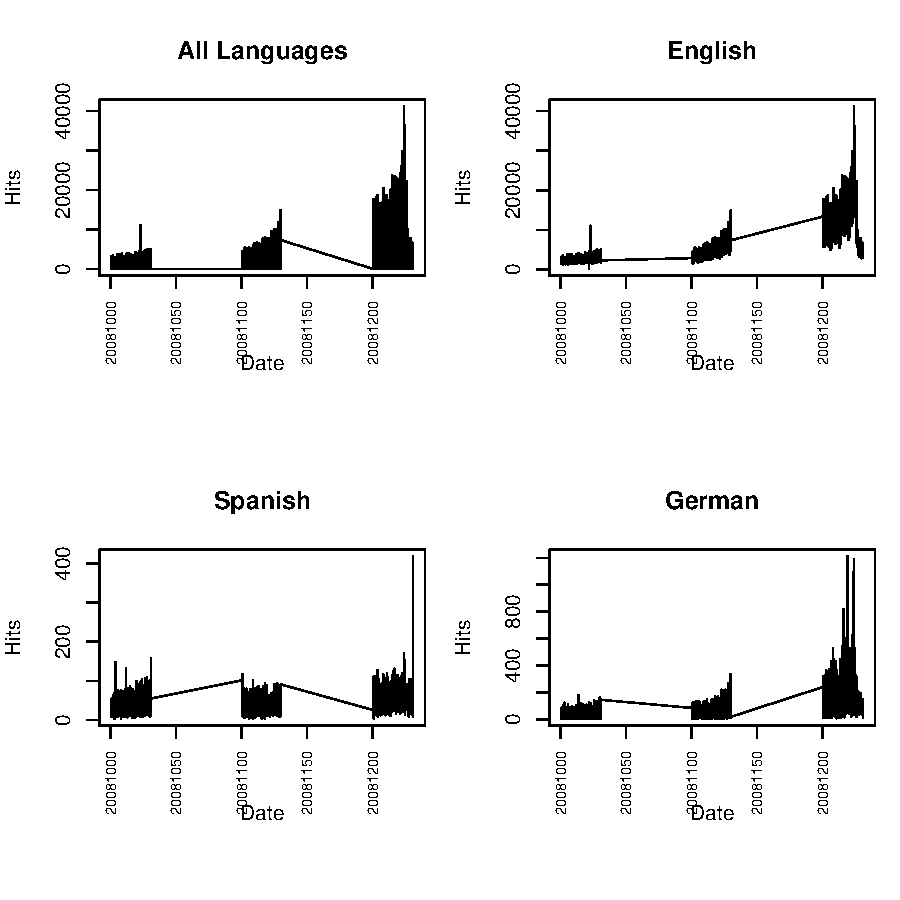
\includegraphics[width=\maxwidth]{figure/unnamed-chunk-6-1} 

\end{knitrout}

I am missing some of the data, not sure why, but I downloaded all hits for "Christmas" for the wikipedia data located in \url{/global/scratch/paciorek/wikistats_full/dated_for_R/}. In the plots you can see that hits for "Chrimstas" grow as time approaches Dec 25, and then sharply drop off towards the end of the year. This is broadly true for all languages and for English, Spanish, and German wikipedia. 

%q4a
\section{This question asks you to complete the exercise begun in ...}


\subsection{Using either foreach or parSapply ...}


Bash code to srun into savio and load r modules
\begin{knitrout}
\definecolor{shadecolor}{rgb}{0.969, 0.969, 0.969}\color{fgcolor}\begin{kframe}
\begin{alltt}
 
# Code to login savio node and load needed R modules
srun -A ic_stat243 -p savio2 --nodes=1 -t 1:00:00 --pty bash
env | grep SLURM  ## see what environment variables are set by SLURM

module load r/3.2.5 doParallel/1.0.10 ggplot2/2.1.0 RColorBrewer/1.1-2 stringr/1.0.0 plyr/1.8.3 dplyr/0.4.3  foreach/1.4.3  
    
#R CMD BATCH --no-save BO_matches.R BO_matches.Rout 
    #I couldn't get R CMD BATCH To work, used R interactively

\end{alltt}
\end{kframe}
\end{knitrout}

R script used to answer quesiton 4a) is below.

\begin{knitrout}
\definecolor{shadecolor}{rgb}{0.969, 0.969, 0.969}\color{fgcolor}\begin{kframe}
\begin{alltt}
\hlcom{####}
\hlcom{# R script}

\hlkwd{rm}\hlstd{(}\hlkwc{list}\hlstd{=}\hlkwd{ls}\hlstd{())}

\hlcom{#load packages}
\hlkwd{require}\hlstd{(readr)}
\hlcom{#Loading required package: readr}

\hlcom{#get files in directory}
\hlstd{dir} \hlkwb{<-} \hlstr{"/global/scratch/paciorek/wikistats_full/dated_for_R/"}
\hlstd{files} \hlkwb{<-} \hlkwd{list.files}\hlstd{(dir)}

\hlcom{#remove uneeded files}
\hlstd{files} \hlkwb{<-} \hlstd{files[}\hlkwd{grepl}\hlstd{(}\hlstr{"part"}\hlstd{, files)]}

\hlcom{#set file paths}
\hlstd{filePaths} \hlkwb{<-} \hlkwd{paste0}\hlstd{(dir, files)}

\hlkwd{head}\hlstd{(filePaths)}
\hlcom{#[1] "/global/scratch/paciorek/wikistats_full/dated_for_R/part-00000"}
\hlcom{#[2] "/global/scratch/paciorek/wikistats_full/dated_for_R/part-00001"}
\hlcom{#[3] "/global/scratch/paciorek/wikistats_full/dated_for_R/part-00002"}
\hlcom{#[4] "/global/scratch/paciorek/wikistats_full/dated_for_R/part-00003"}
\hlcom{#[5] "/global/scratch/paciorek/wikistats_full/dated_for_R/part-00004"}
\hlcom{#[6] "/global/scratch/paciorek/wikistats_full/dated_for_R/part-00005"}

\hlcom{#set read_delim progress bar options}
\hlkwd{options}\hlstd{(}\hlkwc{readr.show_progress} \hlstd{= F)}

\hlcom{#get num cores}
\hlstd{nCores} \hlkwb{<-} \hlkwd{as.integer}\hlstd{(}\hlkwd{Sys.getenv}\hlstd{(}\hlstr{"SLURM_CPUS_ON_NODE"}\hlstd{))}
\hlstd{nCores}
\hlcom{#[1] 24}

\hlkwd{require}\hlstd{(parallel)}
\hlkwd{require}\hlstd{(doParallel)}
\hlkwd{require}\hlstd{(foreach)}

\hlcom{#initialize cores}
\hlkwd{registerDoParallel}\hlstd{(nCores)}

\hlcom{#set iterations}
\hlstd{nSub} \hlkwb{<-} \hlkwd{length}\hlstd{(filePaths)}
\hlstd{nSub}
\hlcom{#[1] 960}

\hlkwd{system.time}\hlstd{(}
\hlstd{result} \hlkwb{<-} \hlkwd{foreach}\hlstd{(}\hlkwc{i} \hlstd{=} \hlnum{1}\hlopt{:}\hlstd{nSub,}
                  \hlkwc{.packages} \hlstd{=} \hlkwd{c}\hlstd{(}\hlstr{"readr"}\hlstd{),}       \hlcom{# libraries to load onto each worker}
                  \hlkwc{.combine} \hlstd{= rbind,}             \hlcom{# how to combine results}
                  \hlkwc{.errorhandling}\hlstd{=}\hlkwd{c}\hlstd{(}\hlstr{"pass"}\hlstd{),}
                  \hlkwc{.verbose} \hlstd{=} \hlnum{TRUE}\hlstd{)} \hlopt \hlstd{\{}

    \hlstd{dat} \hlkwb{<-} \hlstd{readr}\hlopt{::}\hlkwd{read_delim}\hlstd{(filePaths[i],} \hlkwc{delim} \hlstd{=} \hlstr{" "}\hlstd{,} \hlkwc{col_names} \hlstd{= F)}

    \hlkwd{cat}\hlstd{(}\hlstr{"########  iteration "}\hlstd{, i,} \hlstr{" is complete!! :) ########"}\hlstd{)}

    \hlstd{dat[}\hlkwd{grep}\hlstd{(}\hlstr{"Barack_Obama"}\hlstd{, dat}\hlopt{$}\hlstd{X4,} \hlkwc{fixed} \hlstd{= T), ]}
                  \hlstd{\}}
\hlstd{)}
\hlcom{# user    system   elapsed }
\hlcom{#24082.902 72954.630  4497.273}


\hlcom{#check data}
\hlkwd{dim}\hlstd{(result)}
\hlcom{#[1] 430160      6}

\hlkwd{head}\hlstd{(result)}
\hlcom{# A tibble: 6 x 6}
\hlcom{#        X1     X2    X3}
\hlcom{#     <int>  <chr> <chr>}
\hlcom{#1 20081129 210000    pt}
\hlcom{#2 20081014 190000    en}
\hlcom{#3 20081108 190000    no}
\hlcom{#4 20081128 190001    en}
\hlcom{#5 20081110 160000    et}
\hlcom{#6 20081101 110000    fr}
\hlcom{# ... with 3 more variables: X4 <chr>, X5 <int>, X6 <dbl>}



\hlkwd{write.csv}\hlstd{(result,} \hlstr{"/global/home/users/camadams/ps6_BOmatches.csv"}\hlstd{,}
          \hlkwc{row.names} \hlstd{= F,} \hlkwc{quote} \hlstd{= F)}
\end{alltt}
\end{kframe}
\end{knitrout}

It took 4497.273 sec $\sim$ 75 min of "clock" time to run the Barack Obama script on 960 files with 1 node/24cores. 
%4b


\subsection{When I run the Spark code provided with Unit 8, it takes ~15 minutes using 9...}

We can approximate the amount of real time by taking the total kernal time it took to run the barack obama object (user time + system time) and divide it by teh number of processes/cores we are using for the parallel operations. Therefore $(4082.902 + 72954.630 ) / (24 \times 4) = 16.85$ min. This compares favorably to spark, though it is a bit slower. 16.85 min is likely an under estiamte, and it would likely take a little longer than the estimate. 


\begin{knitrout}
\definecolor{shadecolor}{rgb}{0.969, 0.969, 0.969}\color{fgcolor}\begin{kframe}
\begin{alltt}
\hlcom{#Estimate speed of R processes BO data using 96 codes}
    \hlcom{#(user + system time) / cores}
\hlstd{((}\hlnum{24082.902} \hlopt{+} \hlnum{72954.630} \hlstd{)} \hlopt{/} \hlstd{(}\hlnum{24} \hlopt{*} \hlnum{4}\hlstd{))} \hlopt{/} \hlnum{60}
\end{alltt}
\begin{verbatim}
## [1] 16.84679
\end{verbatim}
\end{kframe}
\end{knitrout}


%4c EXTRACT credit
\subsection{Unit 7 discusses the idea of prescheduling ...}
\begin{knitrout}
\definecolor{shadecolor}{rgb}{0.969, 0.969, 0.969}\color{fgcolor}\begin{kframe}
\begin{alltt}
\hlcom{#... same code as in 4a}


\hlcom{#turn off preschedule and employ dynamic allocation}
\hlstd{mcoptions} \hlkwb{<-} \hlkwd{list}\hlstd{(}\hlkwc{preschedule}\hlstd{=}\hlnum{FALSE}\hlstd{)}
\hlstd{nSub} \hlkwb{<-} \hlstd{nSub}\hlopt{/}\hlnum{8} \hlcom{#takes too long to run full data}
\hlstd{nSub}
\hlcom{#120}

\hlkwd{system.time}\hlstd{(}
\hlstd{result} \hlkwb{<-} \hlkwd{foreach}\hlstd{(}\hlkwc{i} \hlstd{=} \hlnum{1}\hlopt{:}\hlstd{nSub,}
                  \hlkwc{.options.multicore} \hlstd{= mcoptions,}
                  \hlkwc{.packages} \hlstd{=} \hlkwd{c}\hlstd{(}\hlstr{"readr"}\hlstd{),}       \hlcom{# libraries to load onto each worker}
                  \hlkwc{.combine} \hlstd{= rbind,}             \hlcom{# how to combine results}
                  \hlkwc{.errorhandling}\hlstd{=}\hlkwd{c}\hlstd{(}\hlstr{"pass"}\hlstd{),}
                  \hlkwc{.verbose} \hlstd{=} \hlnum{TRUE}\hlstd{)} \hlopt \hlstd{\{}

    \hlstd{dat} \hlkwb{<-} \hlstd{readr}\hlopt{::}\hlkwd{read_delim}\hlstd{(filePaths[i],} \hlkwc{delim} \hlstd{=} \hlstr{" "}\hlstd{,} \hlkwc{col_names} \hlstd{= F)}

    \hlkwd{cat}\hlstd{(}\hlstr{"########  iteration "}\hlstd{, i,} \hlstr{" is complete!! :) ########"}\hlstd{)}

    \hlstd{dat[}\hlkwd{grep}\hlstd{(}\hlstr{"Barack_Obama"}\hlstd{, dat}\hlopt{$}\hlstd{X4,} \hlkwc{fixed} \hlstd{= T), ]}
                  \hlstd{\}}
\hlstd{)}
 \hlcom{#user    system   elapsed }
 \hlcom{#4159.053 14686.835   828.382 }
\hlstd{(}\hlnum{828.382} \hlopt{*} \hlnum{8}\hlstd{)} \hlopt{/} \hlnum{60} \hlcom{#120 * 8 = 960 files}
\hlcom{# 6627.056 sec ~ 110 min }

\hlkwd{dim}\hlstd{(result)}
\hlcom{#[1] 54186     6}

\hlkwd{head}\hlstd{(result)}
\hlcom{# A tibble: 6 x 6}
\hlcom{#        X1     X2    X3}
\hlcom{#     <int>  <chr> <chr>}
\hlcom{#1 20081129 210000    pt}
\hlcom{#2 20081014 190000    en}
\hlcom{#3 20081108 190000    no}
\hlcom{#4 20081128 190001    en}
\hlcom{#5 20081110 160000    et}
\hlcom{#6 20081101 110000    fr}
\hlcom{# ... with 3 more variables: X4 <chr>, X5 <int>, X6 <int>}
\end{alltt}
\end{kframe}
\end{knitrout}

Time for static and dyanmic allocation for Barack Obama wikipedia script in R:

\begin{itemize}
    \item[] 4a) Static: $\sim$ 75 min
    \item[] 4c) Dynamic: $\sim$ 110 min
\end{itemize}

Dynamic allocation is slower than static allocation. This is expected here, as each task is expected to take teh same amount of time and use similar computer resources. Dynamic approach sends tasks one at a time to a node, which will increase communication overhead  compared to static allocaiton. Sending a set number of tasks to a core (static) reduces communcation time, and is more efficient when tasks and cores are similar.

%question5 

\section{Details of the Cholesky decomposition presented in Unit 9 ...}

\subsection{Work out the operation count (multiplies and divides) for the Cholesky decomposition ...}

\begin{itemize}
    \item $\alpha_{11} = \sqrt{\alpha_{11}}$ is neglibible
    \item $\alpha_{21} = \frac{\alpha_{21}}{\alpha_{11}} \sim (m - k - 1)$ operations
    \item $A_{22} \sim (m-k-1)^2$ operations
\end{itemize}

Therefore, 

$$\begin{aligned}
\text{Operations } &= \sum_{k=0}^{m-1} (m-k-1)^2 = \sum_{k=0}^{m-1} (m - k - 1) \\
&= \sum_{j=0}^{m-1} j^2 + \sum_{j=0}^{m-1} j \\
&\approx \frac{1}{3}m^3 + \frac{1}{2}m^2 
\end{aligned}$$

\subsection{Suppose I’ve written out the Cholesky calculation based on for loops ...}

Yes, and one would save memory and computational time.

\end{document}






%https://math.stackexchange.com/questions/217738/how-to-calculate-the-cost-of-cholesky-decomposition
%https://www.youtube.com/watch?v=NppyUqgQqd0
%https://rosettacode.org/wiki/Cholesky_decomposition#R
